\chapter{Valutazione}\label{chap:valutazione}

\section{Introduzione al capitolo}\label{sec:intro_cap5}

Nel \cref{chap:implementazione} abbiamo descritto come il sistema sia stato costruito; andremo adesso a valutarne il comportamento. Distinguiamo due piani di analisi: l'\textbf{efficienza} (\cref{sec:efficienza}), ovvero le prestazioni quantitative misurabili (tempo di generazione, tasso di esecuzione corretta, convergenza del training) e l'\textbf{efficacia} (\cref{sec:efficacia}), ovvero il miglioramento qualitativo apportato dal sistema rispetto alle soluzioni precedenti (funzionalità, usabilità e flessibilità).

\subsection{Metodologia generale}\label{subsec:metodologia}

La valutazione quantitativa è stata condotta secondo una pipeline a due fasi, eseguite su macchine diverse per ragioni di disponibilità hardware:


\begin{enumerate}
    \item \textbf{Fase 1 --- Generazione delle predizioni} \\ 
    (\code{generate\_predictions.py}): per ciascuna domanda di un test set di 500 esempi, il modello fine-tuned genera la query SPARQL corrispondente, registrando anche il tempo di generazione per esempio.
    \item \textbf{Fase 2 --- Valutazione contro Blazegraph} \\
    (\code{evaluate\_against\_blazegraph.py}): sia la query generata sia quella di riferimento vengono eseguite contro l'endpoint Blazegraph reale del Datavault, e i rispettivi insiemi di risultati vengono confrontati per calcolare precision, recall e F1.
\end{enumerate}


Abbiamo dovuto dividere la pipeline in due fasi perché la fase di generazione richiede l'accelerazione GPU (non disponibile localmente), mentre la fase di valutazione richiede solo chiamate I/O verso l'endpoint Blazegraph e può essere eseguita comodamente su CPU.\@

\newpage

\subsubsection{Nota metodologica: confronto sull'insieme completo dei risultati}\label{subsec:nota_metodologica}

Una scelta metodologica rilevante riguarda il trattamento delle clausole \code{ORDER BY} e \code{LIMIT}. SPARQL non garantisce un ordine deterministico dei risultati quando è presente un \code{LIMIT} senza un corrispondente \code{ORDER BY}: eseguire due volte la stessa query può restituire campioni diversi delle righe disponibili, producendo falsi negativi anche quando la query generata è testualmente identica a quella di riferimento.

Per questo motivo, precision e recall vengono calcolate sull'insieme \emph{completo} dei risultati, dopo aver rimosso \code{ORDER BY} e \code{LIMIT} da entrambe le query prima dell'esecuzione. L'obiettivo è isolare la correttezza della \emph{logica di filtro} (la clausola \code{WHERE}), cioè se il modello ha capito \emph{quali} elementi cercare, da un controllo distinto sulla clausola \code{LIMIT}: registrato nella colonna \code{limit\_match} del dataset di valutazione, verifica se il modello ha capito anche \emph{quanti} elementi erano richiesti.

% =============================================================================
\section{Efficienza: valutazione quantitativa}\label{sec:efficienza}
% =============================================================================

\subsection{Struttura dei test}\label{subsec:struttura_test}

I parametri di esecuzione del test sono i seguenti:

% \vspace{-0.2cm} % Riduce leggermente lo spazio prima della lista
\begin{itemize}
    \item \textbf{Macchina (generazione)}: GPU NVIDIA T4 (su Kaggle), modello Phi-3-mini fine-tuned con adapter LoRA fuso (\code{merge\_and\_unload}).
    \item \textbf{Macchina (valutazione)}: CPU locale. Nessun modello caricato; esegue unicamente chiamate HTTP verso l'endpoint Blazegraph via proxy Vite.
    \item \textbf{Task}: Traduzione di una domanda in italiano in una query SPARQL, confrontata contro il riferimento generato dal sistema a template (\cref{subsec:dataset_gen}).
    \item \textbf{Dati (Test Set)}: 500 esempi. Costituisce una reale partizione \textit{held-out} (estratta al 5\% con seed deterministico \code{3407}), priva di sovrapposizioni col training.
\end{itemize}

\newpage
\subsection{Distribuzione del test set per categoria}\label{subsec:distribuzione_test}

\vspace{0.5em}

Il test set estratto copre 7 delle 14 categorie di query definite nel generatore (\cref{subsec:dataset_gen}). Come visibile in \cref{tab:distribuzione_test} e \cref{fig:category_distribution}, la distribuzione non è uniforme: la categoria \code{data\_esatta} da sola costituisce quasi la metà del campione (233/500, 46.6\%), mentre alcune categorie di nicchia (es.\@ \code{query\_not\_anno}) non risultano rappresentate. 

Questo sbilanciamento va tenuto presente nell'interpretazione dei risultati: le metriche aggregate sono più informative se lette per categoria (\cref{subsec:metriche_categoria}) che come media generale.

\begin{table}[htbp]
    \centering
    \begin{tabularx}{0.85\textwidth}{X r}
    \toprule
    Categoria          & N. esempi  \\
    \midrule
    \texttt{data\_esatta}        & $233$         \\
    \texttt{formato\_file}       & $66$          \\
    \texttt{fuori\_dominio}      & $57$          \\
    \texttt{dispositivo}         & $40$          \\
    \texttt{container\_cartella} & $30$          \\
    \texttt{ricerca\_testuale}   & $28$          \\
    \texttt{autore}              & $26$          \\
    \texttt{data\_intervallo}    & $20$          \\
    \midrule
    \textbf{Totale}    & \textbf{$500$}\\
    \bottomrule
    \end{tabularx}
    \caption{Distribuzione del test set per categoria euristica.}\label{tab:distribuzione_test}
\end{table}

% --- BLOCCO 2: GRAFICO PGFPLOTS DA CSV (NON fluttuante) ---
\noindent
\begin{minipage}{\textwidth}
    \centering
    \begin{tikzpicture}
    \begin{axis}[
        ybar,
        bar width=14pt,
        width=\textwidth,
        height=7cm,
        ylabel={Numero di esempi},
        xtick={0,1,2,3,4,5,6,7},
        xticklabels={
            \texttt{data\_esatta},
            \texttt{formato\_file},
            \texttt{fuori\_dominio},
            \texttt{dispositivo},
            \texttt{container\_cartella},
            \texttt{ricerca\_testuale},
            \texttt{autore},
            \texttt{data\_intervallo}
        },
        x tick label style={rotate=45, anchor=east, font=\small},
        nodes near coords,
        nodes near coords align={vertical},
        every node near coord/.style={font=\footnotesize},
        ymin=0, ymax=260,
        enlarge x limits=0.12,
        ymajorgrids=true,
        grid style={dashed, gray!30},
    ]
    \addplot[fill={rgb,255:red,70;green,130;blue,180}, draw={rgb,255:red,50;green,100;blue,150}] table[
        x expr=\coordindex,
        y=count,
        col sep=space,
    ] {category_distribution.csv};
    \end{axis}
    \end{tikzpicture}
    \captionsetup{hypcap=false}
    \captionof{figure}{Distribuzione del test set di valutazione $(n=500)$.}\label{fig:category_distribution}
\end{minipage}

% --- TABELLA E GRAFICO AFFIANCATI PER RISPARMIARE SPAZIO ---
% \begin{comment}
%     \begin{figure}[htbp]
%         \centering
%         % Minipage di sinistra per la Tabella
%         \begin{minipage}[c]{0.45\textwidth}
%             \centering
%             \resizebox{0.9\textwidth}{!}{% Adatta la tabella allo spazio della colonna
%             \begin{tabular}{lr}
%             \toprule
%             Categoria & N. esempi \\
%             \midrule
%             data\_esatta        & 233 \\
%             formato\_file       & 66 \\
%             fuori\_dominio      & 57 \\
%             dispositivo         & 40 \\
%             container\_cartella & 30 \\
%             ricerca\_testuale   & 28 \\
%             autore              & 26 \\
%             data\_intervallo    & 20 \\
%             \midrule
%             \textbf{Totale}     & \textbf{500} \\
%             \bottomrule
%             \end{tabular}
%             }
%             \captionof{table}{Distribuzione del test set per categoria euristica.}\label{tab:distribuzione_test}
%         \end{minipage}%
%         \hfill% Spazio flessibile tra tabella e grafico
%         % Minipage di destra per il Grafico
%         \begin{minipage}[c]{0.5\textwidth}
%             \centering
%             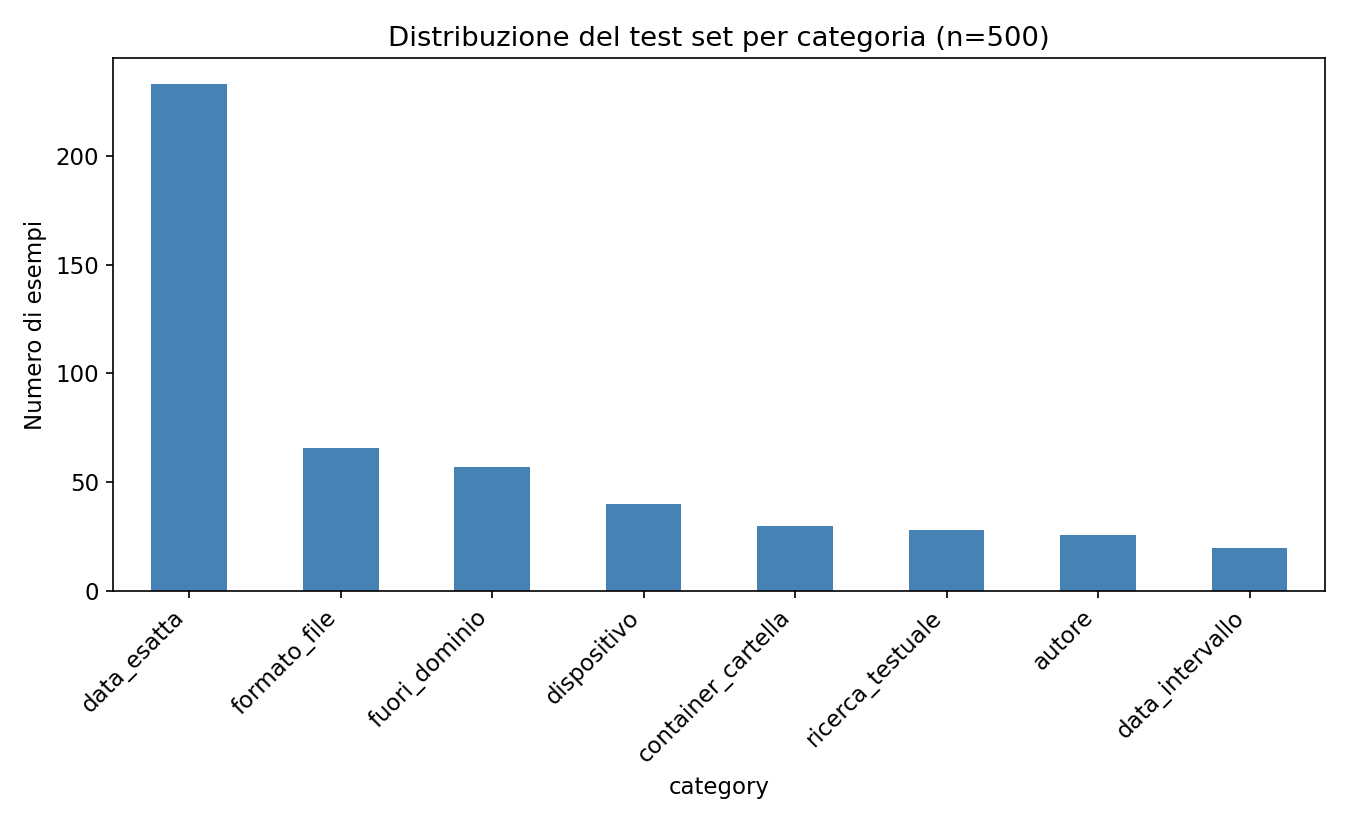
\includegraphics[width=\textwidth]{img/category_distribution.png}
%             % \caption{Distribuzione del test set di valutazione (n=500).}\label{fig:category_distribution}
%         \end{minipage}
%     \end{figure}
% \end{comment}

\newpage
\subsection{Tempo di generazione}\label{subsec:tempo_generazione}

Il tempo di generazione per query, misurato sulla GPU T4 durante la Fase 1, presenta le seguenti statistiche calcolate sull'intero set di 500 esempi:

% --- TABELLA E GRAFICO AFFIANCATI PER RISPARMIARE SPAZIO ---
% \begin{comment}
%     \begin{figure}[htbp]
%         \centering
%         % Minipage di sinistra per la Tabella
%         \begin{minipage}[c]{0.40\textwidth}
%             \centering
%             \begin{tabular}{lr}
%             \toprule
%             Statistica & Valore (s) \\
%             \midrule
%             Media               & 7.45 \\
%             Deviazione standard & 2.51 \\
%             Minimo              & 0.65 \\
%             25° percentile      & 7.64 \\
%             Mediana             & 8.19 \\
%             75° percentile      & 8.59 \\
%             Massimo             & 10.45 \\
%             \bottomrule
%             \end{tabular}
%             % \captionof{table}{Statistiche del tempo di generazione per query (GPU T4).}\label{tab:tempo_generazione}
%         \end{minipage}%
%         \hfill% Spazio flessibile tra tabella e grafico
%         % Minipage di destra per il Grafico
%         \begin{minipage}[c]{0.55\textwidth}
%             \centering
%             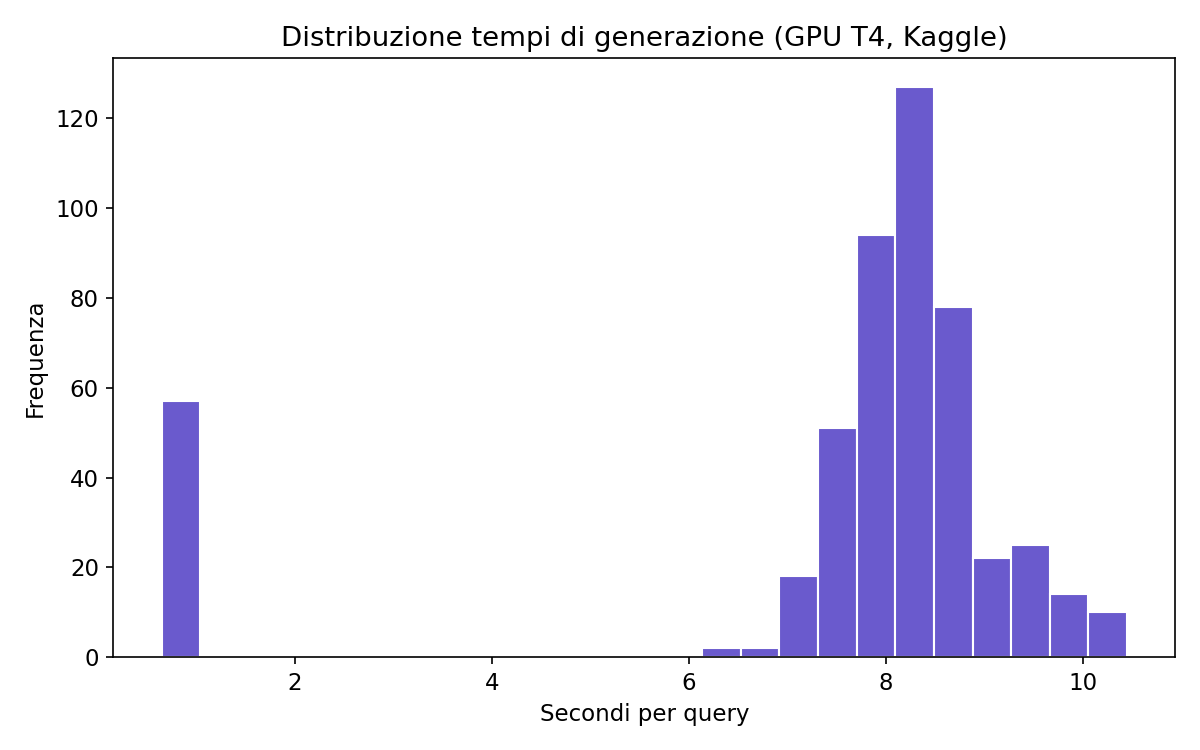
\includegraphics[width=\textwidth]{img/generation_time_hist.png}
%             % \caption{Distribuzione dei tempi di generazione su GPU T4.}\label{fig:generation_time_hist}
%         \end{minipage}
%     \end{figure}
% \end{comment}

\begin{figure}[htbp]
    \centering
    \begin{tabularx}{0.85\textwidth}{X r}
    \toprule
    Statistica & Valore (s) \\
    \midrule
    Media               & 7.45 \\
    Deviazione standard & 2.51 \\
    Minimo              & 0.65 \\
    25° percentile      & 7.64 \\
    Mediana             & 8.19 \\
    75° percentile      & 8.59 \\
    Massimo             & 10.45 \\
    \bottomrule
    \end{tabularx}
    \captionof{table}{Statistiche del tempo di generazione per query (GPU T4).}\label{tab:tempo_generazione}
\end{figure}

\begin{figure}[htbp]
    \centering
    \begin{tikzpicture}
    \begin{axis}[
        ybar interval,
        width=\textwidth,
        height=7cm,
        xlabel={Secondi per query},
        ylabel={Frequenza},
        xmin=0, xmax=11,
        ymin=0,
        minor y tick num=1,
        area style,
        ymajorgrids=true,
        grid style={dashed, gray!30},
        xtick={0,1,2,3,4,5,6,7,8,9,10,11},
        xticklabel style={font=\small},
    ]
    \addplot+[
        hist={bins=22, data min=0, data max=11},
        fill={rgb,255:red,106;green,90;blue,205},
        draw={rgb,255:red,80;green,65;blue,180},
        opacity=0.85,
    ] table [y=time, col sep=space] {generation_times.csv};
    % % Linea verticale per la media
    % \draw[dashed, thick, red!70!black] (axis cs:7.45,0) -- (axis cs:7.45,200)
    %     node[above, font=\footnotesize] {media $= 7{,}45$\,s};
    \end{axis}
    \end{tikzpicture}
    \caption{Distribuzione dei tempi di generazione su GPU T4.}\label{fig:generation_time_hist}
\end{figure}

La distribuzione è concentrata tra i 7 e i 9 secondi per la maggioranza delle query, con una coda di valori bassi (minimo 0.65s) verosimilmente legata a generazioni più brevi, come le risposte \textit{Out-of-Domain}, strutturalmente più corte di una query SPARQL completa.

\subsection{Tasso di esecuzione corretta}\label{subsec:tasso_esecuzione}

Su tutti i 443 esempi non Out-of-Domain del test set, il \textbf{100\% delle query generate è stato eseguito con successo} contro l'endpoint Blazegraph reale, senza errori di sintassi o di esecuzione (\code{execution\_ok = True} per tutte le righe, nessun \code{exec\_error} registrato). Questo risultato conferma, a livello sintattico, l'efficacia delle 8 regole imposte tramite il system prompt (\cref{subsec:regole}) nel vincolare il modello a generare sempre query ben formate.

\subsubsection{Nessun impatto misurato del bug del namespace EXIF}

Il \cref{chap:implementazione} aveva anticipato che l'impatto del namespace EXIF malformato (\cref{subsec:bug_exif_namespace}) sulle metriche di valutazione sarebbe stato verificato in questo capitolo. Il dato è chiaro: \textbf{nessun impatto negativo è stato osservato}. Su 293 dei 443 esempi non Out-of-Domain (categorie \code{data\_esatta}, \code{data\_intervallo} e \code{dispositivo}), la query di riferimento utilizza effettivamente un predicato \code{exif:} nel corpo del \code{WHERE}, non solo nella dichiarazione dei prefissi; tutti e 293 sono stati eseguiti correttamente, con precision e recall pari a 1.000 (\cref{tab:metriche_categoria}).

Questo esito era atteso, ed è la conferma diretta che la strategia di mitigazione descritta nel \cref{chap:implementazione} funziona come previsto: allineando sia il dataset di training sia il backend allo stesso namespace malformato realmente presente in Blazegraph, il sistema evita di generare query che userebbero il namespace standard corretto (\code{www.w3.org}) e fallirebbero sistematicamente. Il bug, di per sé, avrebbe azzerato precision e recall su quasi i due terzi del test set se non fosse stato gestito; il fatto che qui non produca alcun effetto misurabile è merito della scelta di allineamento e non dell'assenza del problema, che resta presente nei dati di produzione e nella fragilità architetturale discussa nel \cref{chap:conclusioni}.

\subsection{Convergenza del training}\label{subsec:convergenza}

Il log di training (\cref{subsec:hyperparams}) mostra una rapida convergenza della loss: da un valore di 0.044 allo step 50 fino a stabilizzarsi attorno a 0.010--0.011 a partire circa dallo step 400, mantenendosi sostanzialmente costante fino al termine dell'addestramento (step 1188, loss finale 0.010).

\begin{figure}[ht]
\centering
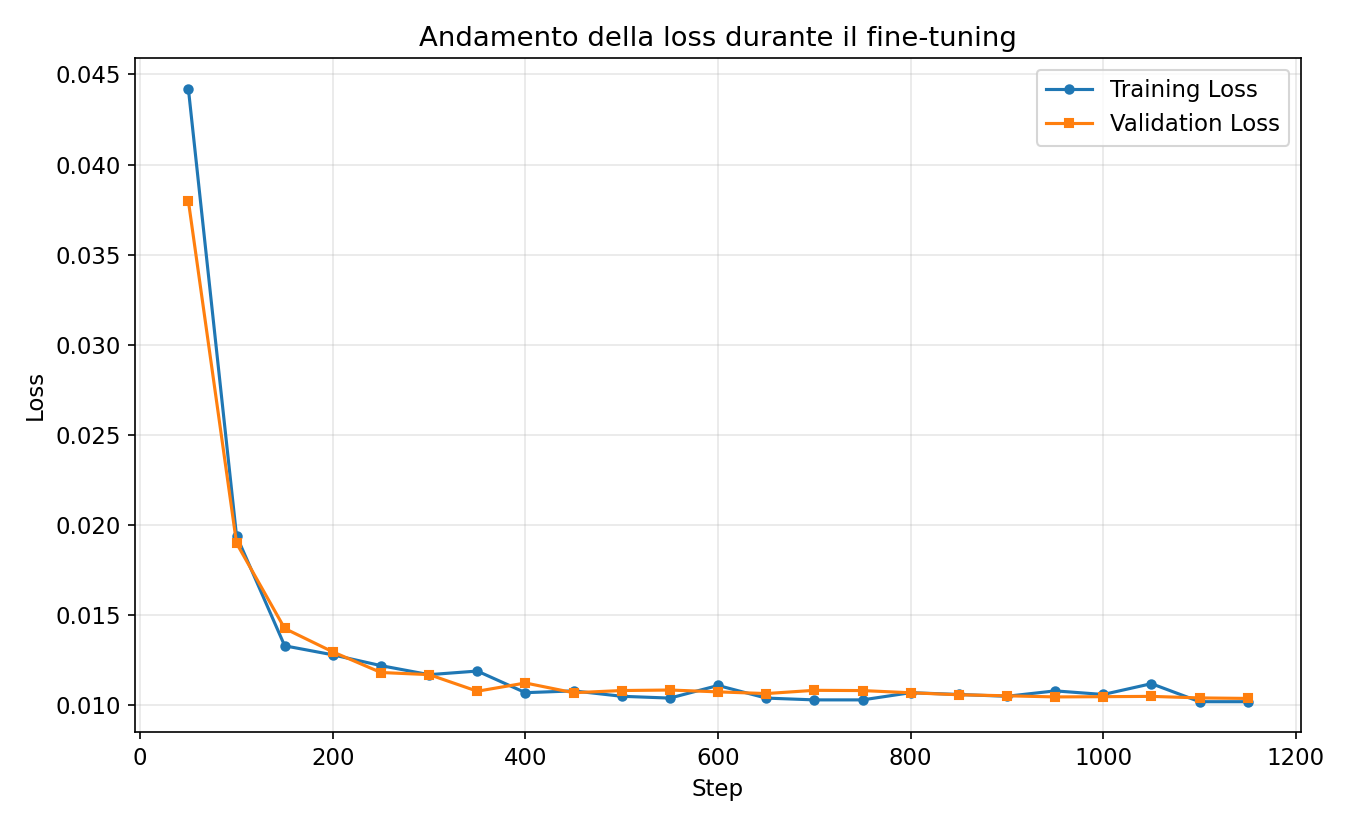
\includegraphics[width=0.85\textwidth]{img/loss_curve.png}
\caption{Andamento della training loss e della validation loss durante il fine-tuning}\label{fig:loss_curve}
\end{figure}

La curva di \textit{validation loss} segue da vicino quella di training, senza divergenze significative: segno di assenza di overfitting. Entrambe le curve si stabilizzano già intorno allo step 400 su un totale di 1188, il che suggerisce che il modello avrebbe potuto convergere anche con meno step.

\newpage
% =============================================================================
\section{Efficacia: valutazione qualitativa}\label{sec:efficacia}
% =============================================================================

\subsection{Metriche di retrieval per categoria}\label{subsec:metriche_categoria}

Applicando la metodologia descritta in \cref{subsec:nota_metodologica}, ovvero il confronto sull'insieme completo dei risultati, al netto di \code{ORDER BY}/\code{LIMIT}, le metriche di precision, recall e F1 per categoria sono le seguenti:

\begin{table}[ht]
\centering
\begin{tabular}{lrrrr}
\toprule
Categoria & N & Precision & Recall & F1 \\
\midrule
data\_esatta        & 233 & 1.000 & 1.000 & 1.000 \\
formato\_file       & 66  & 1.000 & 1.000 & 1.000 \\
dispositivo         & 40  & 1.000 & 1.000 & 1.000 \\
container\_cartella & 30  & 1.000 & 1.000 & 1.000 \\
ricerca\_testuale   & 28  & 1.000 & 1.000 & 1.000 \\
autore              & 26  & 1.000 & 1.000 & 1.000 \\
data\_intervallo    & 20  & 1.000 & 1.000 & 1.000 \\
\midrule
\textbf{Media complessiva} & \textbf{443} & \textbf{1.000} & \textbf{1.000} & \textbf{1.000} \\
\bottomrule
\end{tabular}
\caption{Precision, recall e F1 medi per categoria, calcolati sull'insieme completo dei risultati (al netto di \code{ORDER BY}/\code{LIMIT})}\label{tab:metriche_categoria}
\end{table}

Anche il riconoscimento delle richieste Out-of-Domain (\cref{subsec:errori}) raggiunge il 100\% di accuratezza: tutti i 57 esempi fuori dominio nel test set sono stati correttamente classificati come tali dal modello. Allo stesso modo, il \code{limit\_match} (corrispondenza esatta del valore richiesto nella clausola \code{LIMIT}) è verificato nel 100\% dei 443 casi non Out-of-Domain in cui almeno una delle due query include un \code{LIMIT}.

\subsection{Nota critica: interpretazione dei risultati perfetti}\label{subsec:nota_critica}

I risultati riportati in \cref{tab:metriche_categoria} meritano una discussione esplicita, poiché un punteggio di 1.000 uniforme su ogni metrica e ogni categoria è un esito che richiede cautela interpretativa più che entusiasmo acritico.

Un'ispezione diretta delle 500 coppie (query generata, query di riferimento) in \code{predictions.json} rivela che \textbf{tutte le 500 query generate dal modello sono identiche, carattere per carattere, alla rispettiva query di riferimento}. Questo è un dato di fatto distinto, e più forte, della semplice equivalenza semantica dei risultati: non si tratta di formulazioni sintatticamente diverse che producono lo stesso insieme di risultati, ma di una riproduzione esatta della stringa SPARQL attesa.

Questo fenomeno è spiegabile alla luce di come il test set è stato costruito: le domande e le query di riferimento sono generate dallo stesso sistema di template parametrici (\cref{subsec:dataset_gen}) usato per produrre il dataset di training. Le 8 regole assolute del system prompt (\cref{subsec:regole}) vincolano fortemente la forma sintattica della query attesa: un'unica struttura \code{SELECT DISTINCT ?image WHERE \{\ldots\}}, predicati fissi per ciascun intento, che riduce lo spazio delle risposte plausibili a un insieme ristretto e, per costruzione, deterministico dato l'intento e i parametri della domanda.

In altre parole, una corrispondenza esatta al 100\% è coerente con due ipotesi non mutuamente esclusive:

\begin{enumerate}
    \item Il modello ha effettivamente appreso con grande efficacia la mappatura tra intenti linguistici e struttura SPARQL imposta dalle regole, generalizzando correttamente su parametri (anni, dispositivi, nomi di file) anche se non identici a quelli visti in training;
    \item Il test set, essendo generato dallo stesso processo del training set, condivide con esso una distribuzione di superficie sufficientemente vincolata (per via delle 8 regole assolute) da rendere il compito di generazione quasi deterministico, riducendo il valore di questa valutazione come misura di \emph{generalizzazione} a domande realmente nuove e formulate liberamente da un utente umano.
\end{enumerate}

Il codice di inferenza (\code{generate\_predictions.ipynb}) conferma che il test set costituisce una reale partizione \textit{held-out}: l'estrazione è avvenuta in modo deterministico con un rapporto 95\%/5\% e lo stesso seed (\code{3407}) usato per la configurazione del training. Questo esclude \textit{data leakage} o sovrapposizioni (il modello ha elaborato istanze mai viste in fase di addestramento) e avvalora l'ipotesi della generalizzazione strutturale (punto 1), pur confermando che tale generalizzazione avviene strettamente \textit{in-distribution} rispetto ai template.

Questa osservazione non invalida il risultato: un'accuratezza sintattica ed esecutiva del 100\% sui formati di query coperti dal generatore resta un traguardo solido e utile per l'applicativo. Ne delimita però la portata: la valutazione quantitativa qui presentata misura principalmente la capacità del modello di rispettare in modo affidabile e ripetibile la grammatica e le regole imposte dal system prompt, più che la sua capacità di decodificare formulazioni libere e impreviste di un ricercatore umano. Manca ancora una prova con domande poste in modo spontaneo da utenti reali, non vincolate dai template del generatore (\cref{chap:conclusioni}).

\subsection{Miglioramento rispetto alle soluzioni precedenti}\label{subsec:miglioramento}

Al di là delle metriche quantitative, l'efficacia del sistema si misura anche rispetto al miglioramento qualitativo delle funzionalità disponibili per il ricercatore umanista, in continuità con la discussione del \cref{chap:contesto} (architettura dell'informazione, berrypicking, carico cognitivo):

\begin{sloppypar}
\begin{itemize}
    \item \textbf{Funzionalità}: prima dell'introduzione del sistema, non esisteva alcun meccanismo di ricerca per contenuto o concetto sul Datavault; l'unica modalità di accesso era la navigazione diretta della struttura a container (\cref{subsec:dharc}). Il sistema introduce ex novo questa funzionalità.
    \item \textbf{Usabilità}: l'interazione è ridotta a un singolo campo di testo in linguaggio naturale, eliminando la necessità di conoscere prefissi RDF, sintassi SPARQL o la struttura interna dello schema (\cref{subsec:tre_barriere}).
    \item \textbf{Integrazione}: il sistema si integra nell'infrastruttura esistente (Fedora/Blazegraph) senza richiedere modifiche allo schema dati o migrazioni, operando come layer applicativo aggiuntivo.
    \item \textbf{Manutenzione}: la separazione netta tra dataset di training, system prompt e backend di inferenza (\cref{chap:implementazione}) consente di aggiornare il comportamento del sistema (ad esempio aggiungendo nuove categorie di query) senza dover intervenire sull'infrastruttura dati sottostante.
\end{itemize}
\end{sloppypar}

\subsubsection{Limite: nessun confronto diretto con l'alternativa manuale}

I quattro punti sopra restano un confronto qualitativo basato sull'analisi architetturale del sistema, non su una misura empirica diretta. Non è stato condotto né un cronometraggio del tempo necessario a un utente per scrivere manualmente le query SPARQL dei tre casi d'uso del \cref{chap:prototipo}, né un test di usabilità con ricercatori reali del dominio DH.ARC.\@

Un'indicazione indiretta della differenza attesa viene dalla complessità sintattica stessa dei casi d'uso discussi nel \cref{chap:prototipo}: query come quella del caso d'uso 3 (filtro multi-criterio su dispositivo, intervallo di date e formato) richiedono la conoscenza di almeno tre predicati RDF diversi (\code{exif:make}, \code{exif:dateTime}, \code{ebucore:hasMimeType}) e la sintassi corretta per combinarli in un unico \code{WHERE}, competenze che il profilo utente descritto nel \cref{subsec:utenti} tipicamente non possiede. Questo suggerisce che il vantaggio in termini di tempo e di soglia d'accesso sia sostanziale, ma resta appunto un'aspettativa qualitativa e non un dato misurato.

Colmare questa lacuna con un vero studio comparativo (a tempo, o con un gruppo di utenti reali) è indicato come sviluppo futuro nel \cref{chap:conclusioni}.

% =============================================================================
\section{Discussione dei risultati e limiti della valutazione}\label{sec:discussione}
% =============================================================================

I risultati di questo capitolo si riassumono in tre punti:

\begin{enumerate}
    \item Il sistema è \textbf{sintatticamente affidabile}: il 100\% delle query generate nel test set è eseguibile senza errori contro Blazegraph, grazie al vincolo imposto dalle 8 regole del system prompt.
    \item Il sistema è \textbf{efficiente nei tempi di risposta}: una media di 7.45 secondi per query su GPU T4 è compatibile con un'interazione conversazionale, sebbene il confronto con un'esecuzione su CPU richieda ulteriore verifica empirica (\cref{subsec:tempo_generazione}).
    \item I punteggi di precision/recall/F1 pari a 1.000 vanno interpretati con cautela metodologica (\cref{subsec:nota_critica}): riflettono primariamente la capacità del modello di rispettare un formato di query fortemente vincolato e generato dalla stessa famiglia di template del training set, più che una misura di generalizzazione su domande realmente libere.
\end{enumerate}

Il limite principale di questa valutazione è dunque la natura \textbf{sintetica e in-dominio} del test set utilizzato. Una valutazione più conclusiva richiederebbe un confronto con domande poste da utenti reali del dominio DH.ARC, non vincolate dalla struttura dei template di generazione: un'estensione discussa come sviluppo futuro nel \cref{chap:conclusioni}.

% =============================================================================
\section{Conclusioni del capitolo}\label{sec:conclusioni_cap5}
% =============================================================================

In questo capitolo abbiamo valutato il sistema lungo due assi complementari. Sul piano dell'\textbf{efficienza}, il sistema mostra tempi di generazione contenuti (media 7.45s su GPU), un tasso di esecuzione corretta del 100\% e una rapida convergenza in fase di training (loss stabilizzata già a circa un terzo del training totale). Sul piano dell'\textbf{efficacia}, le metriche di retrieval (precision, recall, F1) raggiungono il valore massimo su tutte le categorie testate: un risultato che, come discusso in \cref{subsec:nota_critica}, va attribuito principalmente all'efficacia delle regole di vincolo sintattico imposte dal system prompt e alla natura in-distribuzione del test set, più che a una dimostrata capacità di generalizzazione su input completamente liberi.

Il \cref{chap:conclusioni} riprende questi risultati per bilanciare i punti di forza del sistema con i suoi limiti noti, e per delineare gli sviluppi futuri necessari a una valutazione più rigorosa e a un utilizzo in produzione del sistema.